\section{Introduction}
\label{sec:intro}
%SSOµÄÌصã
%SSOµÄÏÖ×´

%SSOϵͳµÄ°²È«ÎÊÌ⣬ÐèÒª±£»¤identity proofµÄÍêÕûÐÔ£¬»úÃÜÐÔ£¬°ó¶¨ÐÔ
%ÍêÕûÐÔ£ºÊ¹Óù«¿ªµÄΪÊܱ£»¤µÄÐÅÏ¢×÷Ϊidentity proof
%»úÃÜÐÔ£º±£Ö¤ÓÉIdP·¢Ë͸ø¶ÔÓ¦µÄRP£¬²¢ÇÒ´«Êä¹ý³ÌÖÐͨµÀ¡¢user agent¶¼ÊÇÊܵ½±£»¤µÄ
%°ó¶¨ÐÔ£ºidentity proofÒ»¶¨ÒªÓë¶ÔÓ¦µÄRPʵÏÖ°ó¶¨
%SPRESSOÖйØÓÚimpersonationºÍidentity injectionµÄÃèÊö¡£ Authentication is the most fundamental security property of an SSO system. That is, i) an adversary should not be able to log in to an RP, and hence, use the service of the RP, as an honest user, and ii) an adversary should not be able to log in the browser of an honest user under an adversary¡¯s identity (identity injection).
%Õâ¶ÎÃèÊöÁ½¸öÊÂÇ飺1.secure authentication ¾ÍÊÇÄÜ·ÀסimpersonationºÍidentity injection¡£ È»¶ø£¬ÏÖÔÚÓкܶ๥»÷ʹµÃÕâÁ½¸öÎÞ·¨µÃµ½±£Ö¤¡£¾­¹ý·ÖÎöÖ÷ÒªÊÇÕâÈý¸ö·½ÃæµÄÔ­Òò£º1)RP½ÓÊÜÁËδ±»ÍêÕûÐÔ±£»¤µÄÄÚÈÝ£»2)δ°ó¶¨£»3)й¶¡£
%binding Ô­ÎÄÃèÊö ChenPCTKT14 CCS14 Friendcaster(FriendcasterÊÇÒ»¿îFacebookµÄµÚÈý·½Ó¦Ó㬱ȹٷ½°æµÄ¹¦Äܸü¼ÓÈ«Ãæ) blindly accepting an access token received from a user's device then using this token to exchange for the user's Facebook ID. A malicious application could obtain a legitimate access token from a user, then use this access token to log into Friendcaster as the user. cause they thought Facebook's access tokens were bound to relying parties and checked with every API call: \From Facebook's perspective, the API calls wouldn't appear to be originating from Friendcaster, but the attacker's own app."
%ÍêÕûÐÔÔ­ÎÄÃèÊö IEEE S&P2012 \cite{WangCW12}¹ØÓÚGoogleÎÊÌâÃèÊöwe found that the RPs of Google ID SSO often assume that message fields they require Google to sign would always be signed, which turns out to be a serious misunderstanding (Section 4.1). These problems make us believe that a complete answer to our question can only be found by analyzing SSO schemes on real websites.

% Move to section III
%The primary goal of SSO services is to implement secure user authentication \cite{SPRESSO}, i.e., to ensure that an honest user can always log in to an honest RP under the correct account. To achieve this, an identity proof generated by the IdP should explicitly specify the authenticated user (i.e., \emph{user identification}) and the RP to which the user attempts to log in (i.e., \emph{receiver designation}). The identify proof should be received only by that RP and user but not by any other entities (i.e., \emph{confidentiality}) and verified by the receiver (i.e., \emph{integrity}). However, various attacks exploit vulnerabilities in different SSO systems to break at least one of these requirements \cite{ChenPCTKT14, FettKS16,WangCW12,ZhouE14,WangZLG16,YangLLZH16,SomorovskyMSKJ12,MohsenS16}, where the adversaries attempt to either impersonate the victim user at an honest RP or %manipulate the victim user's browser to log in to honest RPs under the adversary's identity. %(i.e., identity injection). For example, Friendcaster was found to accept any received identity proof \cite{ExplicatingSDK,ChenPCTKT14} (i.e., a violation of receiver designation) so that a malicious RP could log in to Friendcaster as the victim user by replaying the identity proof received from the user to Friendcaster \cite{MohsenS16}. \cite{WangCW12} reported that some RPs of Google ID SSO accepted user attributes that were not tied to the identity proof (i.e., a potential violation of integrity). As a result, a malicious user could insert arbitrary attributes (e.g., an email address) into the identity proof to impersonate another user at the RP.


%SSO ÒýÈëеÄÒþ˽ÎÊÌâ
%IdPÖªµÀÓû§µÇ¼ÄĸöRP
%RPÖ®¼ä¿ÉÒÔºÏı֪µÀͬһ¸öÓû§µÇ¼ÄÄЩRP
Single sign-on (SSO) protocols such as OpenID Connect (OIDC) \cite{OpenIDConnect}, OAuth 2.0 \cite{rfc6749} and SAML \cite{SAML,SAMLIdentifier}, are widely deployed in the Internet for identity management and authentication.
With the help of SSO, a user logins to a website, referred to as the \emph{relying party} (RP), using his identity registered at a trusted web service, known as the \emph{identity provider} (IdP).
An RP delegates user identification and authentication to the IdP, which issues an \emph{identity token} (e.g., id token in OIDC or identity assertion in SAML) for a user to visit the RP. %after authenticating this user.
%Moreover, SSO shifts the burden of user authentication from RPs to IdPs and reduces security risks and costs at RPs.
%Besides,
%    the user only manages his attributes at the IdP,
%        but not one copy for each RP.
%
%SSO has been widely integrated into many application services. For example, 80\% of the Alexa Top-100 websites and 6.3\% of the Alexa Top-1M websites support SSO \cite{GhasemisharifRC18}. Meanwhile, many email and social network providers (such as Google, Facebook, Twitter, etc.) are serving the IdP roles.
%
For example, in common OIDC systems, a user sends a login request to the target RP. % (Step 1),
Then, the RP constructs an identity-token request with its identity (denoted as $ID_{RP}$) and redirects this request to the IdP.
After authenticating the user,
 the IdP issues an identity token explicitly binding the identities of both the user and the RP (i.e., $ID_U$ and $ID_{RP}$),
    which is returned to the user and forwarded to the RP. %in Step 5.
Finally, the RP verifies the identity token to decide whether the user is allowed to login or not.
So, a user keeps only one credential for the IdP, instead of several credentials for different RPs.

As the comprehensive solution of identity management and authentication,
    SSO services allow the IdP to provide more attributes in the tokens
        along with the authenticated user's identity.
The attributes (e.g., age, hobby, education, and nationality) are maintained at the IdP,
    and enclosed in the identity tokens after the user's authorization \cite{OpenIDConnect,rfc6749}.

%However, SSO systems have been continuously found vulnerable and insecure \cite{WangCW12,ccsSunB12,SomorovskyMSKJ12,ArmandoCCCPS13,DiscoveringJCS,dimvaLiM16,WangZLG16,MainkaMS16, MainkaMSW17,YangLCZ18}.
The wide adoption of SSO raises concerns on user privacy \cite{maler2008venn,NIST2017draft,BrowserID,SPRESSO},
 because SSO facilitates curious parties to track a user's login activities.
To issue identity tokens,
in each login instance
 the IdP is aware of when and to which RP a user attempts to login.
As a result, an honest-but-curious IdP could track all the RPs that each user has visited over time \cite{BrowserID,SPRESSO},
% This data can be further analyzed to profile users' online activities, as in other web tracking attacks.
 called {\em IdP-based login tracing} in this paper.
%This threat by curious IdPs is also discussed by recent researches .
Meanwhile, the RPs learn users identities from the identity tokens.
If the IdP encloses the same user identity in the tokens when the user visits different RPs \cite{Google, FirefoxAccount},
     collusive RPs could link these login instances across the RPs %and track the user's activities
      and learn the user's online profile \cite{maler2008venn}.
We denote this privacy risk as {\em RP-based identity linkage}.
%These privacy threats result from the designs of SSO protocols \cite{NIST2017draft},
%     but not any specific implementations of SSO services.

%This threat is usually mitigated by pairwise pseudonymous identifiers (PPIDs) in practice \cite{NIST2017draft,OpenIDConnect, SAMLIdentifier}.
%Popular SSO protocols leak user privacy in different ways,

%
%%As SSO becomes a popular safeguard for various privacy-sensitive web services, the privacy concern is considered more prominent and severe than it was in the past.
%Recently, many IdPs have taken user privacy in SSO into serious consideration and offered new protection against RP-based identity linkage.
%For example, Figure \ref{fig:wechat} shows the IdP service provided by WeChat, one of the most popular instant messaging applications in China.
%It allows a user to create new accounts with new profile attributes to log in to different RPs.
%Similarly, IdPs such as NORDIC APIS and CURITY suggest adopting pairwise pseudonymous identifier (PPID) in SSO \cite{Nordic, Curity},
% and Active Directory Federation Services \cite{MS} and Oracle Access Management \cite{Oracle} support the use of PPID.

%However, these efforts cannot protect users from IdP-based login tracing.
%While privacy-savvy users may provide few personal information to web applications to avoid user tracking or profiling,
% the use of popular SSO services such as Google Account opens a door for IdPs and application providers to recover users' online traces and profiles,
%  which makes users' privacy protection effort in vain.
%Several large IdPs, especially the social IdPs, are known to be interested in collecting users' online behavioral data for various purposes
% (e.g., Screenwise Meter \cite{googlenews} and Onavo \cite{Onavo}).
%Serving the IdP role makes it possible for them to collect such information.
%Finally, privacy-preserving record linkage \cite{agrawal2003information} and
% private set intersection \cite{de2010practical} technologies allow multiple RPs to share data without violating the privacy policies,
% which pave the path for cross-organizational RP-based identity linkage.
%Or even service providers hosting multiple web applications take an advantaged position to correlate users' multiple logins
% at different RPs through internal information integration.
%%%%%%%%%% ×¢Ò⣬ÎÒÃDz¢²»ÄÜ´¦ÀíIdPºÍRPÖ®¼äµÄºÏı¹¥»÷
%
%\begin{figure}[t]
%  \centering
%  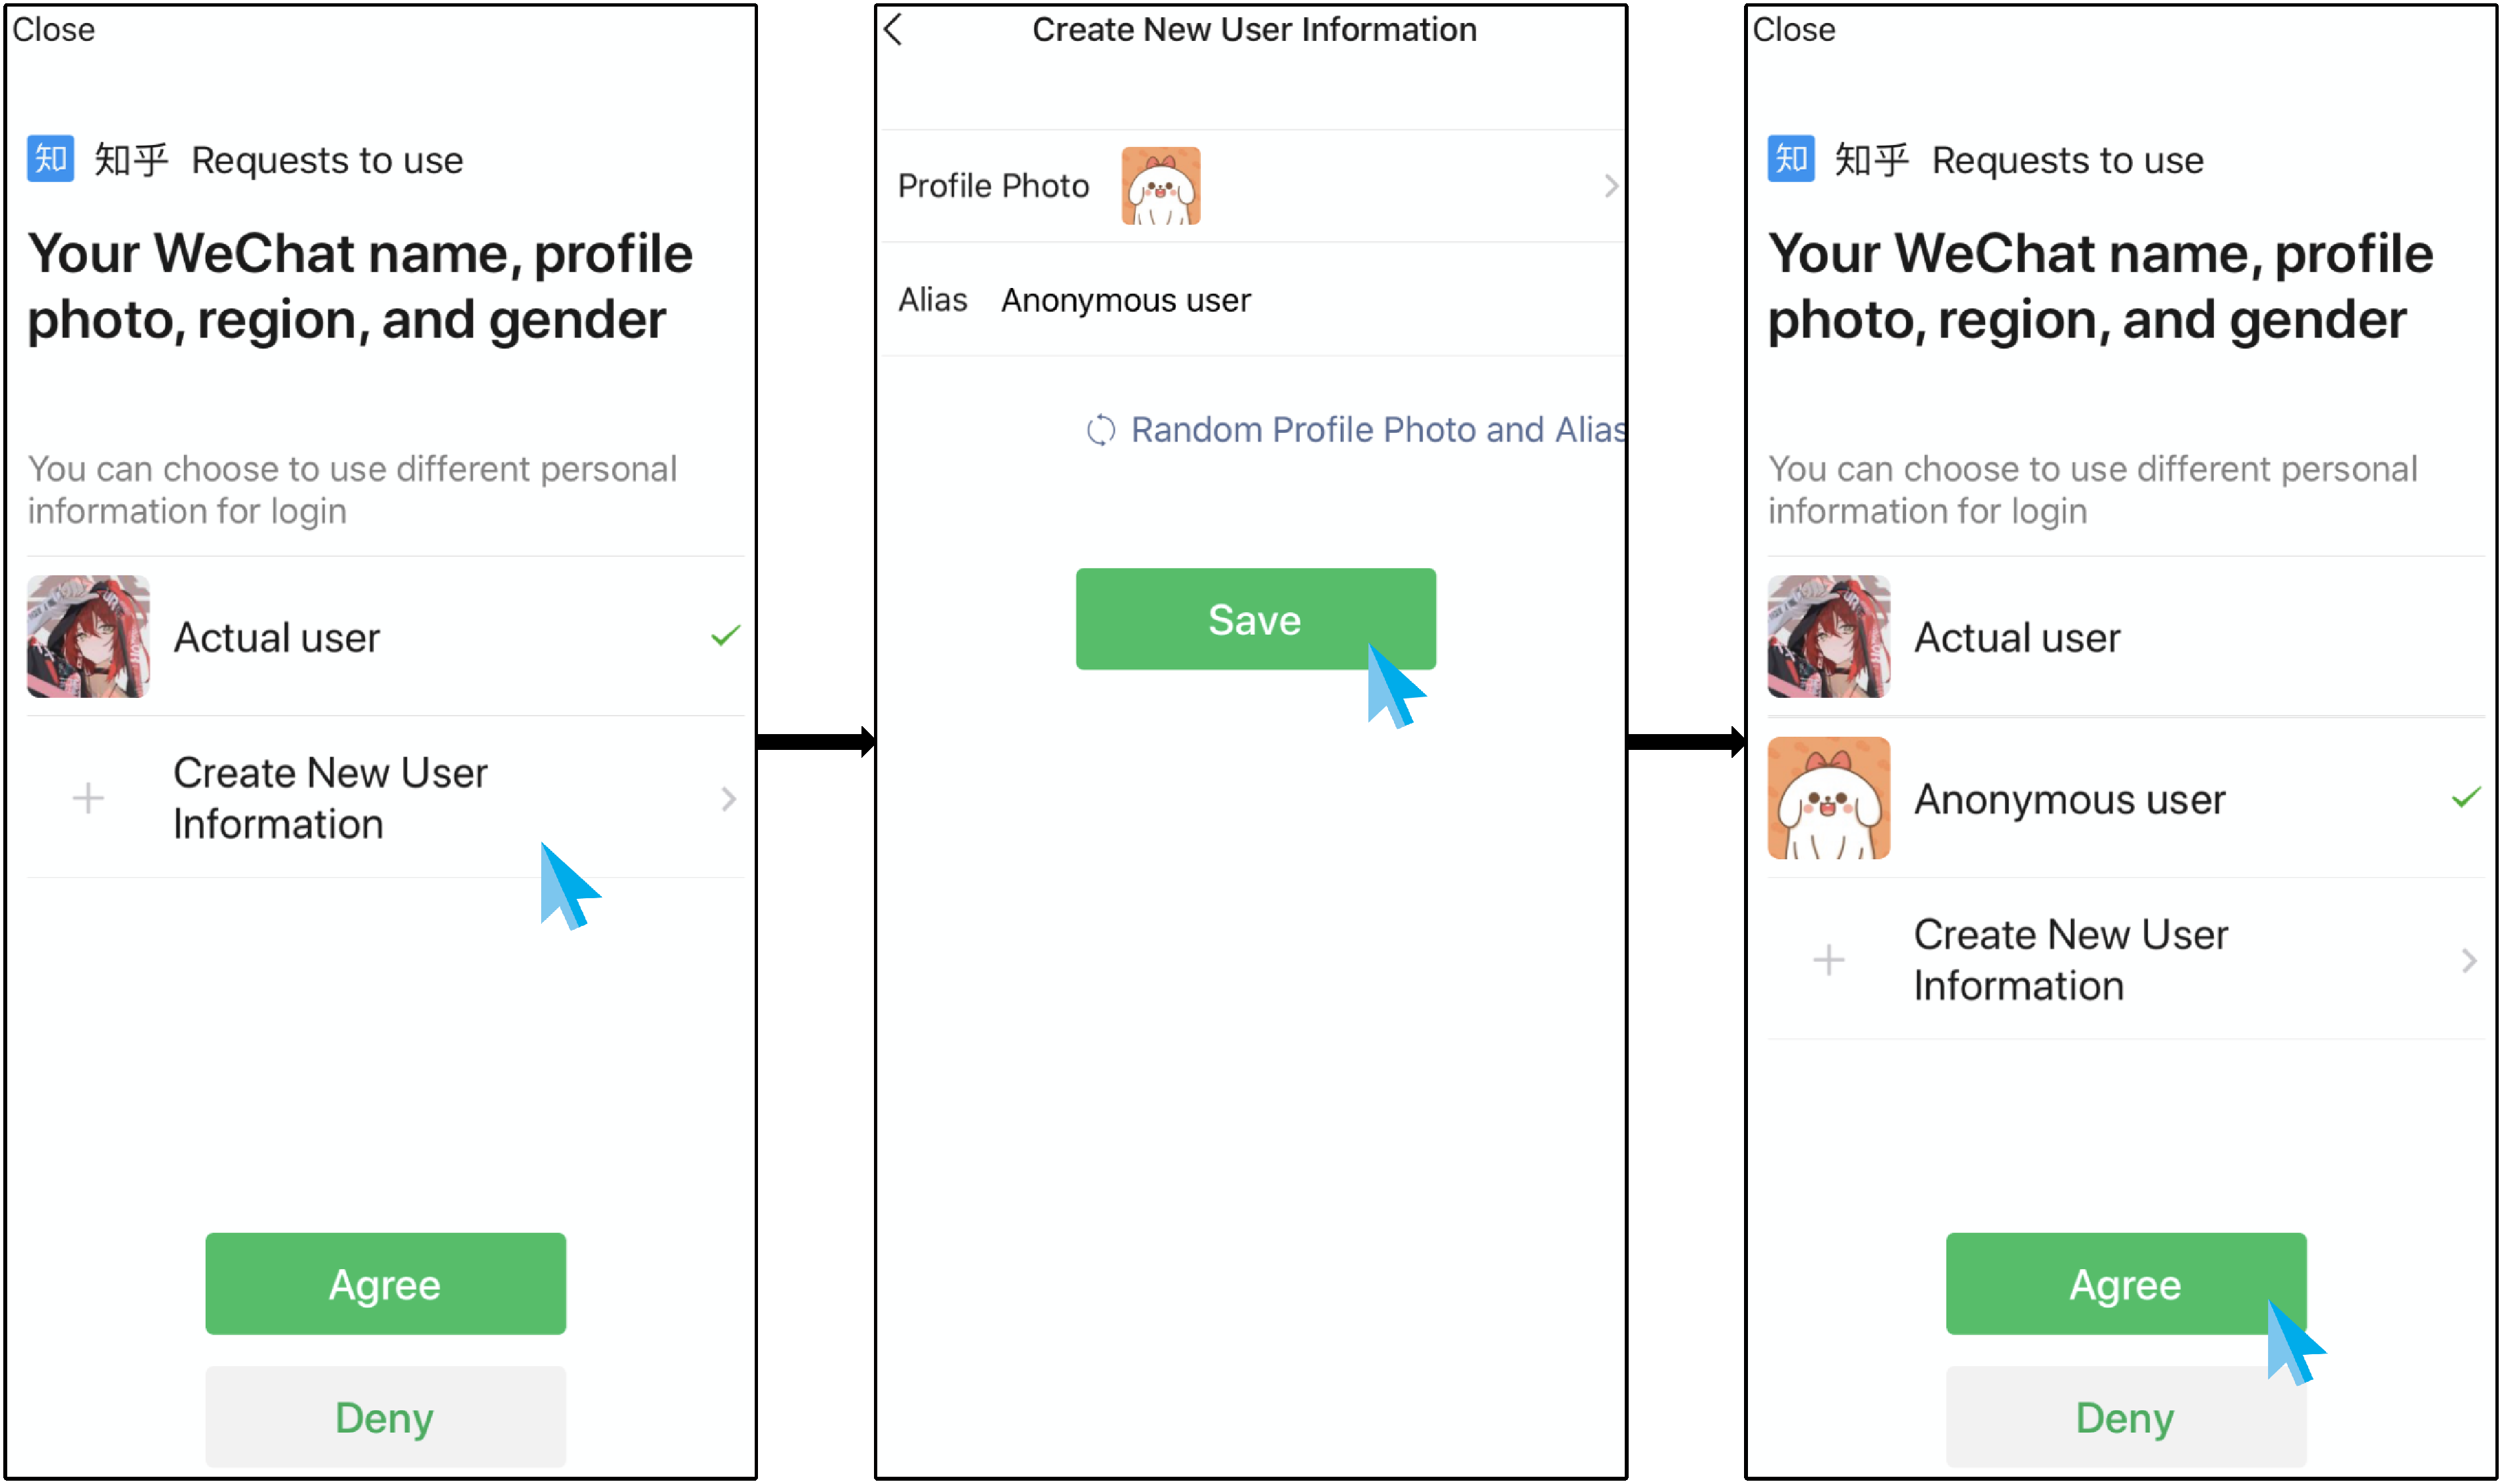
\includegraphics[width=0.9\linewidth]{fig/wechat.pdf}
%  \caption{Anonymous SSO login in WeChat.}
%  \label{fig:wechat}
%  \vspace{-5mm}
%\end{figure}

%also raises privacy concerns regarding online user tracking and profiling.
%Imagine that, a user concerning her privacy would avoid to leave her full sensitive information at an application. The user may use multiple web applications and only leave parts of her sensitive messages at each applications, for example, using  real name on social website, the address on shopping website and the phone number on Telecom website. And she would try not to leave any linkable message to avoid applications combining her informations, for example, if she leave the email on each applications, they can combine the parts of informations through the email. However,  the privacy leaks in SSO systems make her effort in vain. As long as a user employs the SSO system, such as Google Account, to log in to these applications, the applications providers and Google can combine your informations based on the SSO account.

%google and facebookµÄ¸ºÃæÐÂÎÅ
%1. service provider£¨ÈçDNS£©ÖªµÀÄã·ÃÎÊÁË£¬¿ÉÒÔ´øÀ´ºÜ¶àÎÊÌâ¡£µ«ÊÇ»¹ÊDz»Í¬µÄ£¬DNSÀïprofileÐèÒªÆÀ¹ÀµÄÊÇtwo behavior vectorsµÄsimilarities£¬¶øIdPÖж¼²»ÐèÒª£¬ÒòΪIdPÄܹ»Çø·Ötwo behavior vectors ÊÇ·ñÀ´×ÔÏàͬ½Úµã¡£


Privacy-preserving SSO schemes are expected to support comprehensive identity management and authentication while protecting user privacy \cite{maler2008venn,NIST2017draft,BrowserID,SPRESSO}.
Therefore, they should provide the following design features:
(\emph{a}) \emph{User identity at an RP},
    i.e., an identity token enables an RP to uniquely identify every user,
(\emph{b}) \emph{User authentication only to the IdP}, i.e.,
    the steps of authentication between a user and the RP are eliminated,
    and a user only needs to hold the secret credential to authenticate himself to the IdP,
%    different types of credentials are supported in the authentication between the IdP and users,
and (\emph{c}) \emph{Provision of IdP-confirmed user attributes}, i.e., a user maintains his attributes at the trusted IdP and RP-requested attributes are provided %with the user's identity
after authorized by the user.
Meanwhile, the privacy threats from different types of adversaries are considered: (\emph{a}) \emph{honest-but-curious IdP}, (\emph{b}) \emph{collusive RPs}, and (\emph{c}) \emph{honest-but-curious IdP colluding with some RPs}.
In Section \ref{subsec-solutions}, we overview the existing privacy-preserving SSO solutions and identity federation.


%However, to the best of our knowledge,
% {\em none of them provides a practical protection against both the IdP-based login tracing and the RP-based identity linkage}
%  (see Sections \ref{subsec-solutions} and \ref{sec:related} for details).
%The techniques proposed so far to defend against each of the two threats cannot be integrated,
%    for they require modifications to the SSO login flows that essentially conflicts.
%This requires a non-trivial re-design of SSO protocols against the threats of user privacy,
%while providing secure identity management and authentication.

We conceptualize the privacy requirements of SSO into
  an {\em identity transformation} problem %and explain the reasons that limit existing solutions from fully protecting user privacy against both curious IdPs and collusive RPs.
and propose an Untraceable and Unlinkable Privacy-PREserving Single Sign-On (UPPRESSO) protocol to protect user privacy.
In particular, we design three identity-transformation functions for the SSO login flow.
In each login instance, the RP transforms its $ID_{RP}$ to an ephemeral $PID_{RP}$ for the requesting user and sends it to the IdP, who then transforms $ID_U$ to an ephemeral $PID_U$ accordingly. Hence, the identity token binds ephemeral IDs %($PID_U$ and $PID_{RP}$) 
instead of the permanent ones. %($ID_U$ and $ID_{RP}$).
Finally, after receiving an identity token with the matching $PID_{RP}$, the RP transforms $PID_U$ into a user ``account'', which remains identical across multiple login instances. Meanwhile, a user's accounts at different RPs are different and unrelated.
%Given a user, this account is identical across multiple login instances and unique at each RP.

Unlike existing privacy-preserving SSO solutions~\cite{BrowserID,SPRESSO,NIST2017draft} that prevent only one of the two privacy threats, 
UPPRESSO can eliminate both of them. 
%On the contrary, existing privacy-preserving SSO \cite{BrowserID,SPRESSO,NIST2017draft} prevents only one of these two privacy threats.
It prevents {\em IdP-based login tracing} by hiding the RP's permanent identity from the IdP %sees only $PID_{RP}$ in the identity-token request 
during the login process and {\em RP-based identity linkage} by constructing unique yet consistent user accounts at each RP.
The identity transformations work compatibly with the login flows of widely-adopted SSO protocols~\cite{OpenIDConnect,rfc6749,SAML,NIST2017draft} so that UPPRESSO supports all desired security features of SSO. %the benefits of SSO protocols are kept in UPPRESSO.
 %       and it is very easy to implement UPPRESSO on top of OIDC systems.
%
%
%This prevents both IdP-based login tracing by hiding the RPs' identities from the IdP and RP-based identity linkage by hiding the user's identity from the RPs.
%Meanwhile, an RP is still able to link multiple login sessions of the same user by converting the user's different pseudo-identities to an invariant user account using a special identifier-transformation function and the trapdoors, without knowing the user's real identity in the IdP.
% Finally, we formally prove that the accounts of the same user at different RPs are independent and cannot be correlated by collusive RPs (see our proof in Section \ref{sec:privacy}).
%UPPRESSO designs three one-way identifier-transformation functions based on elliptic curve cryptography. Using the one-way trapdoor function $\mathcal{F}_{ID_{RP} \mapsto PID_{RP}}(ID_{RP}, T)$, the RP converts its identity $ID_{RP}$ into a privacy-preserving pseudo-identity $PID_{RP}$ based on a randomly selected trapdoor $T$. Similarly, the IdP uses the one-way function  $\mathcal{F}_{ID_{U} \mapsto PID_{U}}(ID_U, PID_{RP})$ to generate a privacy-preserving pseudo-identity $PID_U$ for the user based on her identity $ID_U$ and $PID_{RP}$. Finally, using a special identifier-transformation function $\mathcal{F}_{PID_{U} \mapsto Account}(PID_U, PID_{RP}, T)$, the RP is able to map all the different privacy-preserving pseudo-identities of a user, which are created in her different login sessions to that RP, to a same $Account$ that identifies the user to the RP. The three identifier-transformation functions work cooperatively to ensure: (\emph{a}) when a user logs in to an RP multiple times, the RP can always map $PID_U$s to a unique $Account$ without knowing the user's identity $ID_U$; moreover, when a user logs in to multiple RPs, (\emph{b}) a curious IdP learns nothing about the identities of these RPs from $PID_{RP}$s, and (\emph{c}) collusive RPs cannot link $PID_U$s to a particular user %or associate them together, (\emph{d}) nor correlate $Account$s of a same user at different RPs.
%
%While keeping the features of popular SSO,
%UPPRESSO prevents both the IdP-based login tracing and the RP-based identity linkage,
%    by the identity-transformation functions during the generation of identity tokens
%    and the calculation of accounts.
%
We summarize our contributions as follows.
\vspace{-\topsep}\begin{itemize}
\setlength{\topsep}{0pt}
\setlength{\partopsep}{0pt}
\setlength{\itemsep}{0pt}
\setlength{\parsep}{0pt}
\setlength{\parskip}{0pt}
\item We formalize the SSO privacy problems as an identity-transformation challenge and propose a  solution to protect users' login activities;
that is, solve this challenge by designing identity-transformation functions.
\item
The UPPRESSO protocol is presented based on identity transformations with several designs specific for web applications.
We prove that UPPRESSO satisfies all the security and privacy requirements of the SSO services.

%To the best of our knowledge, UPPRESSO is the first practical SSO system against both the IdP-based login tracing and the RP-based identity linkage.

%\item We formally prove the privacy of UPPRESSO based on the DDH assumption \cite{GoldwasserK16} and the security of UPPRESSO based on a formal model of the web infrastructure. Our results show that UPPRESSO provides expected and satisfying security and privacy protection to SSO.
%provide the reduction from UPPRESSO scheme to DDH Assumption proving that it is protected from IdP-based login tracing and RP-based identity linkage,
%and analyze the security of UPPRESSO based on a formal model of the web infrastructure and formally prove that it provides satisfying security properties.
\item
We build a prototype system for web applications on top of an open-source OIDC implementation. With experimental performance evaluations, we show that UPPRESSO introduces reasonably small overheads.
\end{itemize}

The remainder is organized as below.
Section \ref{sec:background} presents
    the background and related works.
The identity dilemma of privacy-preserving SSO is analyzed  in Section \ref{sec:challenge},
    and Section \ref{sec:UPPRESSO} presents the designs of UPPRESSO.
Security and privacy are analyzed in Section \ref{sec:analysis}.
We explain the prototype implementation and experimental evaluations in Section \ref{sec:implementation},
 and discuss extended issues in Section \ref{sec:discussion}.
Section \ref{sec:conclusion} concludes this work.

